\begin{frame}{Заключение}

\begin{footnotesize}

Работа над этой презентацией не окончена. Актуальная версия расположена по~адресу
\url{http://mech.math.msu.su/~shvetz/54/inf/metapost/mpshort.pdf}.

При создании настоящего руководства использовались следующие технологии:
\hologo{LuaLaTeX}, \hologo{METAPOST}.

\bigskip

\begin{columns}
\column{.115\textwidth}
\centering
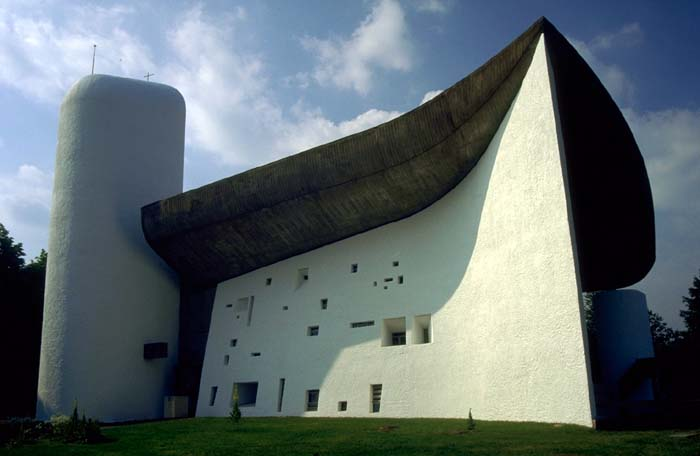
\includegraphics[width=.96\textwidth]{figure-ronchamp}
\column{.835\textwidth}
Изображение капеллы \textfrench{Notre Dame du~Haut} в~Роншане архитектора
Ле~Корбюзье (Le~Corbusier) взято по~адресу
\url{http://home.broadpark.no/~lhellemo/gallery/architecture/Le_Corbusier_front.jpg}
\end{columns}

\medskip

\begin{columns}
\column{.115\textwidth}
\centering
\scalebox{.3}{\includeMPgraphics{figure-mmflogo}}
\column{.835\textwidth}
Логотип механико"=математического факультета МГУ имени М.~В.~Ломоносова
первоначально был создан С.~В.~Голованем в~системе~\hologo{METAFONT}
и~адаптирован автором для \hologo{METAPOST}.
\end{columns}

\medskip

\begin{columns}
\column{.115\textwidth}
\centering

\includegraphics[width=.96\textwidth]{aiga_hotel_information1}
\column{.835\textwidth}
Пиктограммы взяты с~сайта \url{http://aiga.org}.
\end{columns}

\medskip

\begin{columns}
\column{.115\textwidth}
\centering
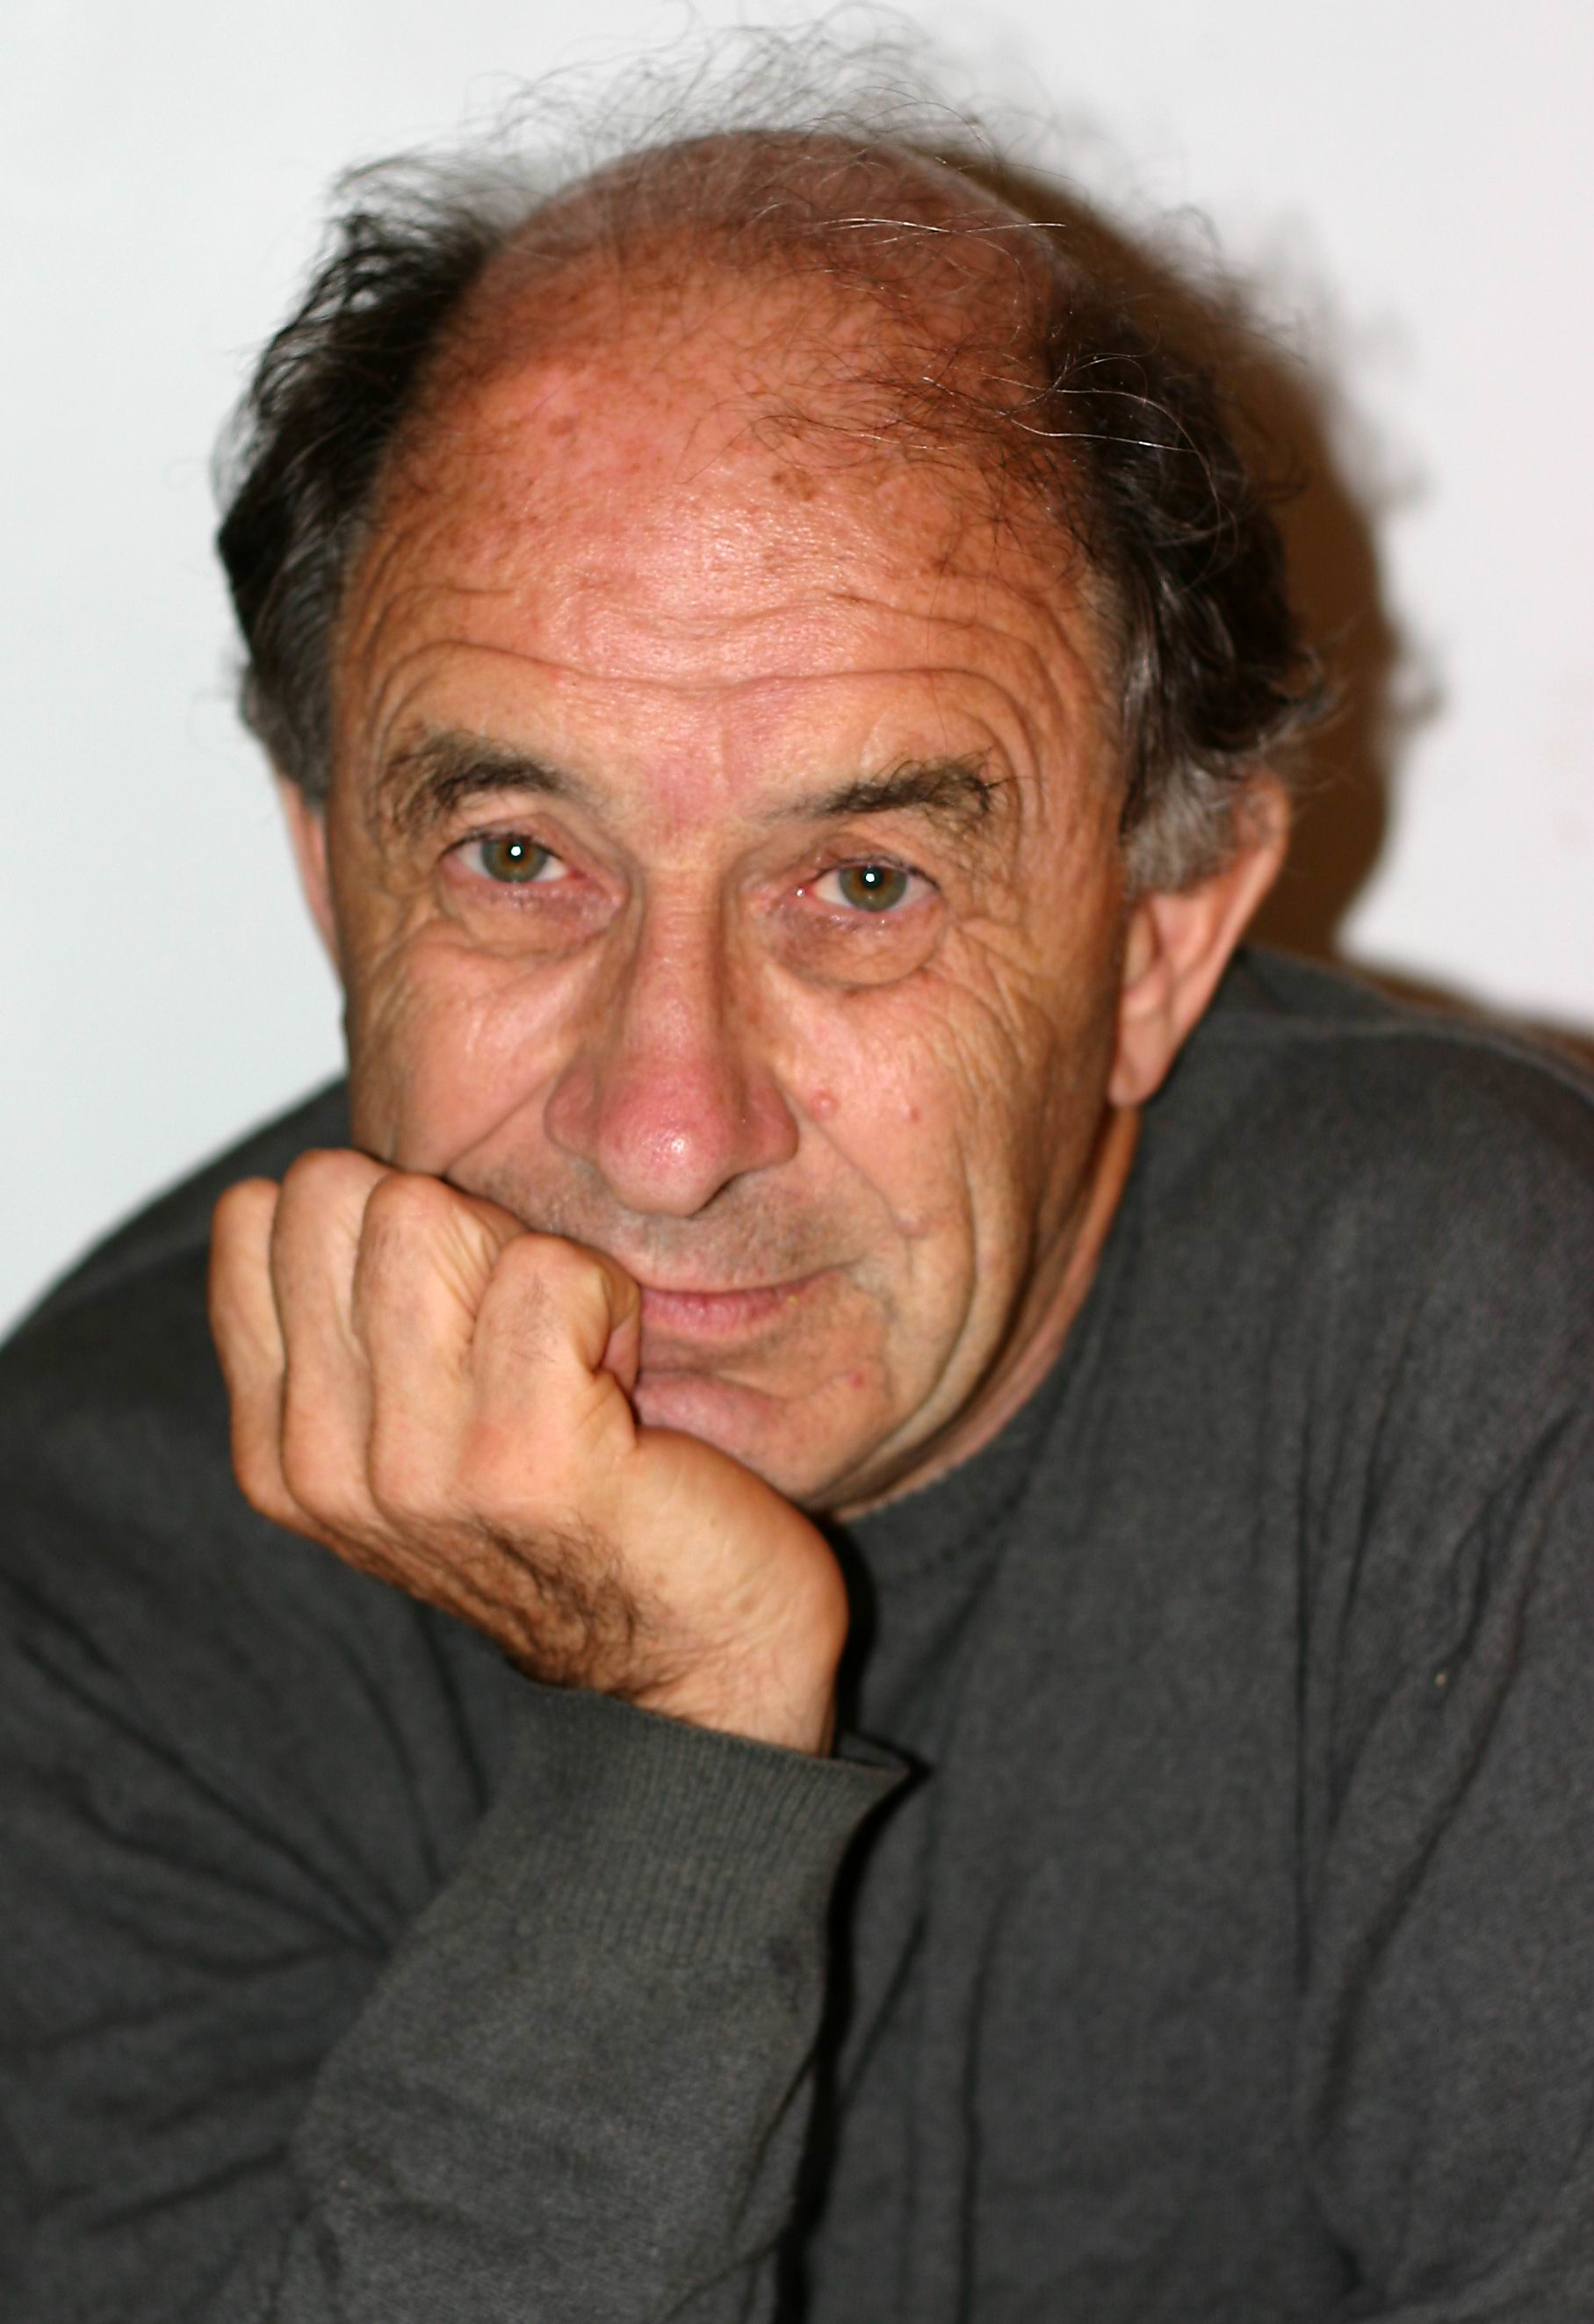
\includegraphics[width=.6\textwidth]{figure-arnold}
\column{.835\textwidth}
Фотография В.~И.~Арнольда взята на Википедии:
\url{https://commons.wikimedia.org/wiki/File:Vladimir_Arnold-1.jpg}.
\end{columns}

\end{footnotesize}
\end{frame}

\begin{frame}

\vskip0pt plus1filll

%\begin{center}
{\Huge\itshape
Спасибо за внимание!}
%\end{center}

\vskip0pt plus1filll

\begin{itemize}
\tiny
\item[\hbox to2em{\hfil{\fontspec{FontAwesome}^^^^f25e}\hfil}]
\href{https://creativecommons.org/licenses/by-sa/4.0/deed.ru}
%{{\usebeamerfont{normal text}{\nolinkurl{CC-BY-SA-4.0 License}}}}
{{\usebeamercolor[fg]{math text}CC-BY-SA-4.0 License}}
\item[\hbox to2em{\hfil{\fontspec{FontAwesome}^^^^f0c1}\hfil}]
\url{http://mech.math.msu.su/~shvetz/54/inf/metapost/mpshort.pdf}
\item[\hbox to2em{\hfil{\fontspec{FontAwesome}^^^^f09b}\hfil}]
\url{https://github.com/urbic/mpshort}
\item[\hbox to2em{\hfil{\fontspec{FontAwesome}^^^^f1d2}\hfil}]
\expandafter\href{https://github.com/urbic/mpshort/commit/\githash}{\nolinkurl{\githash}}
\item[\hbox to2em{\hfil{\fontspec{FontAwesome}^^^^f199}\hfil}]
\href{mailto:shvetz.anton@gmail.com?subject=mpshort}{\nolinkurl{shvetz.anton@gmail.com}}
\end{itemize}
\vspace{3ex}
\end{frame}
